\chapter{Models for \Ttwo relaxation enhancement}\label{ch:models}

As discussed in Chapter \ref{ch:background}, researchers have developed a number of models to explain the decrease in \Ttwo of the water protons in blood.
Thulborn originally applied the Luz-Meiboom equation to describe the decrease in \Ttwo and its dependence on the CPMG echo time\cite{ThulbornOxygenationdependencetransverse1982}.
This assumes that the water protons in blood exchange between two sites with different Larmor frequencies, with a rate $\frac{1}{\tau_{ex}}$.
While this provides good agreement with experimental data, it does not provide a good description of the underlying physical system - for example, the exchange time in found in previous studies do not agree with other measurements of the exchange rate across the red blood cell membrane \cite{Herbstreviewwaterdiffusion1989}.
There are also inconsistencies in the values of $\tau_{ex}$ reported in the literature, with values ranging from 0.3 ms to 10.1 ms (see \autoref{tab:dm-litTex}).
Another model has been proposed by Jensen and Chandra, which more describes the dephasing of water protons that diffuse through areas of magnetic field inhomogeneities\cite{JensenNMRrelaxationtissues2000}.
Generally, the two models predict the same behaviour at short echo times (\textless 3 ms) and at long echo times (\textgreater 20ms)\cite{BrooksT2shorteningweaklymagnetized2001}, but in the intemediate range, the two models give different values for the magnitude of the \Ttwo change.
Additionally, experiments comparing the two models have found that at clinical MRI fields (1.5 T and up), both models provide good agreement with experimental data \cite{StefanovicHumanwholebloodrelaxometry2004,ChenHumanwholeblood2009,GardenerDependencebloodR22010,GrgacHematocritoxygenationdependence2013}.
Because of this, the Luz-Meiboom equation is typically used when analysing data, as it is simpler than the diffusion model.

It is also possible that both mechanisms are occuring together, in which case, it is useful to know the relative contributions of the two processes.
Based on studies of the spectroscopic line width of red blood cell suspensions, Matwiyoff et al. suggest that diffusion processes dominate at higher fields, while exchange between cytoplasm and plasma is more significant at lower fields (\textless 1.5 Tesla)\cite{Matwiyofflineshapeswater1990}.
As another component of this research, the agreement between these models and data collected at lower fields has been tested to investigate whether the different models are more effective at lower field.

\begin{table}[h]
\centering
\caption{Previous studies of \Ttwo shortening and dependence on exchange time}
\label{tab:dm-litTex}
\begin{tabular}{|llll|}
\hline
Author     & Year & Field (T) & Tex (ms)      \\
\hline
Thulborn   &   1982\cite{ThulbornOxygenationdependencetransverse1982}  & 4.2       & 0.6           \\
Gomori     &   1987\cite{GomoriNMRRelaxationTimes1987}  & 0.94      & 9.1 \pm 0.1   \\
Bryant     &   1990\cite{BryantMagneticrelaxationblood1990}  & 1.4       & 10            \\
Brooks     &   1995\cite{BrooksComparisont2relaxation1995}  & 1.0       & 3.4           \\
Meyer      &   1995\cite{MeyerNMRrelaxationrates1995}  & 4.7       &  1  \\
Stefanovic &   2004\cite{StefanovicHumanwholebloodrelaxometry2004}  & 1.5       & 3.0 \pm 0.2   \\
Chen       &   2009\cite{ChenHumanwholeblood2009}  & 3         & 1.67 \pm 0.01 \\
Gardener   &   2010\cite{GardenerDependencebloodR22010}  & 2.35      & 4.4 \pm 0.4   \\
Gardener   &   2010\cite{GardenerDependencebloodR22010}  & 7         & 4.4 \pm 2.1 \\ \hline
\end{tabular}
\end{table}

\section{Theory}
Thulborn proposed using the Luz-Meiboom equation to describe the decrease in \Ttwo that occurs in deoxygenated blood in the CPMG experiment.
This equation comes from the study of a chemical exchange process, where protons on an ammonium ion exchange with the solvent\cite{LuzNuclearMagneticResonance1963}.
Protons bound to the ammonium ion have a different chemical shift, which combined with the exchange, makes the refocusing pulses in the CPMG experiment less effective.
Luz and Meiboom show that this process leads to a \Ttwo decrease dependent on the echo time given by \autoref{eq:LMchemEx}\cite{LuzNuclearMagneticResonance1963}, where $p_i$ is the fraction of protons in state $i$, $\delta_i$ is the shift of protons in state $i$, $t_{ec}$ is the echo time, and $\tau_{ex}$ is the average time between exchanges. It also includes the $T_{20}$ to include the $T_2$ when there is no exchange contribution.

\begin{equation}
\label{eq:LMchemEx}
\frac{1}{T_2} = \frac{1}{T_{20}} + \sum_i{p_i\delta_i^2} (1 - \frac{t_{ec}}{2\tau_{ex}} \tanh{\frac{2\tau_{ex}}{t_{ec}}})
\end{equation}

\begin{equation}
\label{eq:LMblood}
\frac{1}{T_2} = \frac{1}{T_{20}} +(P_A)(1 - P_A)\tau_{ex} \left[(1-sO_2)\alpha\omega_0\right]^2 \left(1 - \frac{\tau_{ex}}{t_{ec}} \tanh{\frac{\tau_{ex}}{t_{ec}}}\right)
\end{equation}

This was thought to be a similar situation to red blood cells, where the susceptibility change due to haemoglobin causes a difference in the field in the cytoplasm compared to the plamsa, and protons exchange across the cell membrane.
One version of this interpretation is given by Wright\cite{WrightEstimatingoxygensaturation1991}. In \autoref{eq:LMblood} the summation over the states becomes $P_A$, which is the relative population of protons in cytoplasm and plasma (and therefore the haematocrit, and the frequency difference given by a term dependent on the $sO_2$, the field strength $\omega_0$, and a dimensionless factor $\alpha$ which is dependent on the susceptibility change of deoxyhaemoglobin.

One challenge to applying this model comes from the term $\tau_{ex}$.
In the literature, there are a range of values for the exchange time - see \autoref{tab:dm-litTex}.
This is typically attributed to using different ranges of $t_ec$ in the CPMG experiments, which can cause the fitting to become biased.
In addition, many of these do not agree with values for the rate of transmembrane exchange when measured by other NMR methods (Typically > 10 ms\cite{Herbstreviewwaterdiffusion1989}.)
This suggests that the exchange time parameter is not necessarily due to exchange across the cell membrane.

A similar formula has been found by Jensen and Chandra, following a more general derivation of the signal in CPMG experiments from protons diffusing in a weakly inhomogeneous field\cite{JensenNMRrelaxationtissues2000}.
Their model uses the weak field approximation, which requires a correlation function $K(t)$ that describes the variations in the magnetic field as protons diffuse.
By approximating this correlation function with a simple exponential decay, they found that the relaxation rate is given by \autoref{eq:LMsimp}\cite{JensenNMRrelaxationtissues2000}.
This has the same form as the Luz-Meiboom formula, but with the exchange time replaced by a more general ``correlation time'', and the factor $K_0$ representing the variance of the magnetic field.
Because of this, their correlation time is not directly connected to an exchange process, which could explain why the Luz-Meiboom formula agrees with experimental results, but also gives a range of exchange times.
\begin{equation}
\label{eq:LMsimp}
\frac{1}{T_2} = \frac{1}{T_{20}} + \gamma^2 K_0 (1 - \frac{2\tau_{ex}}{t_{ec}} \tanh{\frac{2\tau_{ex}}{t_{ec}}})
\end{equation}

By using a different correlation function which describes the diffusion of water molecules around microscopic field inhomogeneities, Jensen and Chandra also derived another formula for the change in \Ttwo.

\begin{equation}
\label{eq:JC}
\frac{1}{T_2} = \frac{1}{T_{20}}+ G_0 \frac{\gamma^2 r_c^2}{2D} F(\frac{4D \Delta t}{r_c^2})
\end{equation}

\begin{displaymath}
\mbox{where  } F(x) = \frac{1}{\sqrt{\pi}} \int_0^\infty \frac{e^{-y}}{\sqrt{y}} \left[1-\frac{1}{xy} \tanh{xy}\right] \mathrm{d}y
\end{displaymath}
Here, $G_0$ is the mean squared magnitude of field inhomogeneities, $r_c$ is their characteristic length scale (i.e. the size of the red blood cells), and $D$ is the diffusion coefficient of water protons.
In studies comparing the two models, it has been shown that the two models agree well enough with experimental data, but differ slightly in the range

\section{Experimental Setup}
To better map out the dependency of \Ttwo on echo time, a wider range of echo times than the 5 used in the other continuous experiments was required.
In this series of experiments, a new pulse sequence  was written to sequentially measure multiple CPMG experiments using a range of echo times specified by the user.
The pulse sequence supports either using a linear range of echo times, or loading a file with the desired echo times.
A list of 13 times between 0.5 - 20 ms was used, with more closely spaced samples in the region between 1 - 5 ms, as this is where the differences in the predictions of the two models are most visible.
To ease processing, the number of echoes in each CPMG experiment is the same.
This presented a problem with measuring longer echo times, for example, 200 echoes at 20 ms requires an experiment time of 4 seconds.
Overall, the experiment with 13 echo times, and a T\textsubscript{R} of 5 seconds takes 5 minutes.
This was repeated to collect two data sets at each field strength, from the same blood sample.

These experiments were completed during the continuous flow experiments, with experiments done at each field strength.
Because of the difficulties found when trying to maintain intermediate levels of blood oxygenation (e.g. in the stopped flow experiments), experiments were done using blood in a deoxygenated state (see \autoref{tab:dm-fitPars}).
Deoxygenated blood was typically used in the literature, and creates stronger contrast in the \Ttwo effect, due to the increased field inhomogeneities.
The oxygenation was logged by optical sensor, and found to vary <3\% over the experiment.
The same flow rate from the continuous flow experiments was maintained using the screw clamp, which meant that the blood did not have the chance to settle and meant that the temperature was relatively stable during the 5 minutes of the experiment ( \mbox{$\pm 4^{\circ}\, \mathrm{C}$}) TODO see how much this actually was!!.

\subsection*{Analysis method}
To compare the two models, a similar approach was used to Stefanovic and Pike\cite{StefanovicHumanwholebloodrelaxometry2004}, Chen and Pike \cite{ChenHumanwholeblood2009} and Gardener and colleagues\cite{GardenerDependencebloodR22010}.
\Ttwo values were calculated for each echo time using least squares fitting of the phased and integrated echo amplitudes with the function $S=Ae^{(t/T_2)}$.
To remove the effect of the fast decaying signal from the tube surrounding the blood, the first 40 ms of the CPMG decay is ignored in the fitting.
Data from after 1 s was also excluded, as it was found that the signal from the blood has decayed by this time, leaving only noise that biased the fitting.
The average of \Ttwo values from the two experiments was used to fit to constrained versions of equations \ref{eq:LMsimp} and \ref{eq:JC}  (where either $\tau_{ex}$ or $r_c$ are held constant).
In these cases $\tau_{ex}$ was set to 3.0 ms, and $r_c$ set to 4.30 um, which were the values found by Stefanovic and Pike at 1.5T\cite{StefanovicHumanwholebloodrelaxometry2004} (the closest values field where this type of experiment has been done.)
Their experiments typically held \TtwoO constant in the constrained models, but this would not have allowed for changes in intrinsic \Ttwo due to haemolysis or other changes in the state of the blood which we know occurs in these experiments, so this was used as a second fitted parameter.
In all fits, the diffusion coefficient of water was was assumed to be $D = 2.0 \mu m^2 ms^{-1}$.
The results from the constrained fit were then used as initial guesses for an unconstrained least squares fit to the formulae, where all three parameters were allowed to vary.
This was needed to ensure the curve fitting procedure converged.
Finally, the Sums-of-Squared-Residual (SSR) was calculated to give a quantitative measure of the model's agreement with the measured data.

\section{Results}

\subsection{\Ttwo Measurement}
CPMG decays were measured for blood in the contunuous flow setup at each of the field strengths used in those experiments.
To obtain a \Ttwo value for each echo time, the echo intensities were fit to a monoexponential decay.
An example of this is shown in \autoref{fig:dm-CPMGdecay}, the section of the decay used for fitting is also marked.

\begin{figure}[h]
\centering
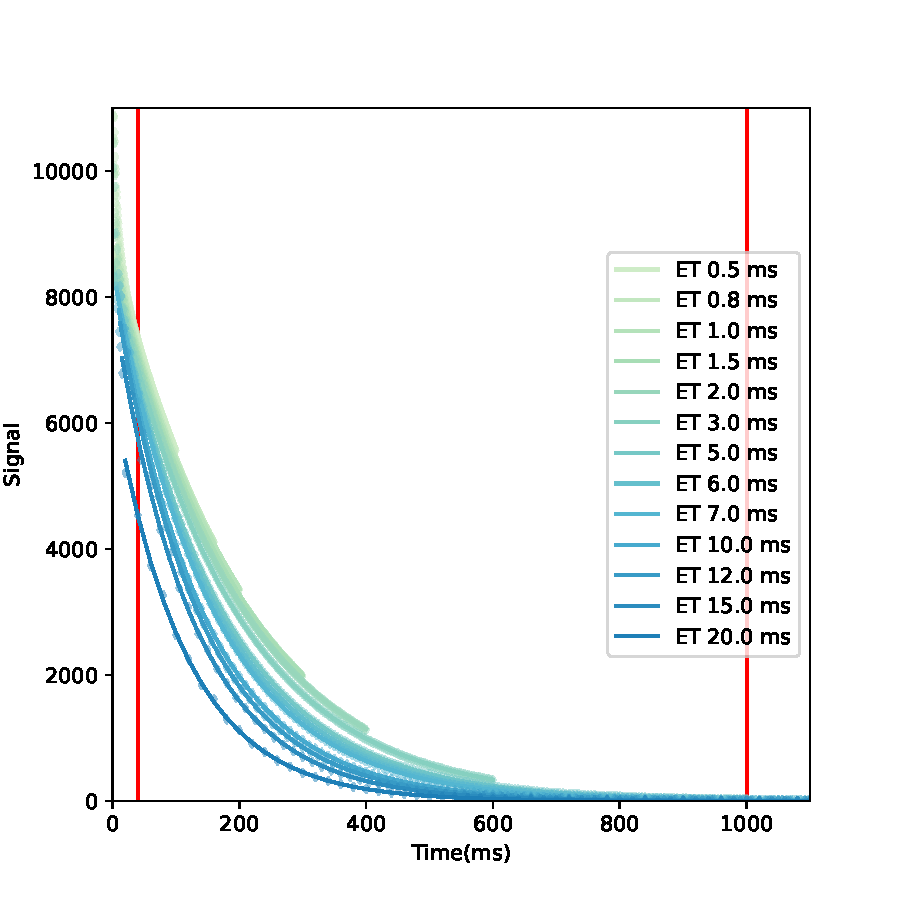
\includegraphics[width=10cm]{figures/diffmodels/20MHzT2fit.pdf}

\caption{CPMG decays measured at the field of 20 MHz, at the different echo times. Red lines indicate data points used for fitting}
\label{fig:dm-CPMGdecay}
\end{figure}

With the exception of the fast decay from the plastic tube at the start of the CPMG experiment, the echo intensities show good agreement with the monoexponential decay function, which confirms that the blood is not separating, and that the decay is not significantly affected by the flow.

\subsection{Model fitting}

Values of \Ttwo measured at each echo time were then used as inputs for fitting equations \ref{eq:LMsimp} and \ref{eq:JC}.
Errors from the \Ttwo fitting are on the order of 2 ms.
The resulting best fit curves for both equations are shown in \autoref{fig:dm-fitResults}, while the parameters are included in \autoref{tab:dm-fitPars}.

\begin{table}[h]
\centering

\caption[Best fit values to the experimental data at different fields]{Best fit values to the experimental data at different fields, shaded columns indicate fixed parameters in fitting. Note that the \TtwoO values are going to be dependent on the state of the blood in the flow circuit, so are not necessarily reflective of the diffusion/exchange effects.}
\label{tab:dm-fitPars}


\makebox[\textwidth][c]{
\begin{tabular}{l|cccr|cccr|}
%Copied from Python/processCPMGvt/newCPMGvt
& \multicolumn{4}{c}{Constrained LM} & \multicolumn{4}{c}{Unconstrained LM} \\ Field 
& T\textsubscript{20} & K\textsubscript{0} & Tau\textsubscript{ex} \cellcolor[gray]{0.8} & SSR
& T\textsubscript{20} & K\textsubscript{0} & Tau\textsubscript{ex} & SSR\\
 & ms & 10\textsuperscript{-14} T\textsuperscript{2} & ms \cellcolor[gray]{0.8} & ms\textsuperscript{2}& ms & 10\textsuperscript{-14} T\textsuperscript{2} & ms & ms\textsuperscript{2}\\ \hline
40 MHz & 227 \pm 4.2 & 7.081 \pm 0.162 & 3.00 \cellcolor[gray]{0.8} & 3733 & 248 \pm 5.8 & 8.445 \pm 0.311 & 2.08 \pm 0.11 & 1199\\
20 MHz & 219 \pm 1.6 & 2.832 \pm 0.022 & 3.00 \cellcolor[gray]{0.8} & 277 & 210 \pm 1.9 & 2.459 \pm 0.048 & 3.55 \pm 0.08 & 498\\
14 MHz & 297 \pm 0.5 & 0.868 \pm 0.005 & 3.00 \cellcolor[gray]{0.8} & 410 & 298 \pm 0.5 & 0.990 \pm 0.020 & 2.30 \pm 0.08 & 183\\
10 MHz & 294 \pm 1.5 & 0.473 \pm 0.023 & 3.00 \cellcolor[gray]{0.8} & 616 & 305 \pm 3.3 & 0.654 \pm 0.062 & 1.96 \pm 0.18 & 89\\
5  MHz & 277 \pm 2.2 & 0.392 \pm 0.025 & 3.00 \cellcolor[gray]{0.8} & 443 & 283 \pm 3.2 & 0.588 \pm 0.092 & 1.81 \pm 0.30 & 177\\

%stop copying

\end{tabular}
}

\vspace{1cm}

\makebox[\textwidth][c]{
\begin{tabular}{l|cccr|cccr|}

%Same deal..
& \multicolumn{4}{c}{Constrained JC} & \multicolumn{4}{c}{Unconstrained JC} \\ Field 
& \TtwoO & \Gzero & \rc \cellcolor[gray]{0.8} & SSR
& \TtwoO & \Gzero & \rc & SSR\\
 & \si{ms} & \SI{e-14}{T^2} & \si{\micro\metre} \cellcolor[gray]{0.8} & \si{ms^2} & \si{ms} & \SI{e-14}{T^2} & \si{\micro\metre} & \si{ms^2}\\ \hline
40 MHz & 253 \pm 5.2 & 9.985 \pm 0.217 & 4.30 \cellcolor[gray]{0.8} & 844 & 272 \pm 8.6 & 11.643 \pm 0.636 & 3.58 \pm 0.19 & 120\\
20 MHz & 225 \pm 1.7 & 3.932 \pm 0.031 & 4.30 \cellcolor[gray]{0.8} & 56 & 220 \pm 2.4 & 3.588 \pm 0.105 & 4.65 \pm 0.12 & 34\\
14 MHz & 299 \pm 0.5 & 1.227 \pm 0.007 & 4.30 \cellcolor[gray]{0.8} & 88 & 300 \pm 0.6 & 1.393 \pm 0.044 & 3.70 \pm 0.12 & 35\\
10 MHz & 301 \pm 1.9 & 0.748 \pm 0.036 & 4.30 \cellcolor[gray]{0.8} & 181 & 309 \pm 4.4 & 1.022 \pm 0.161 & 3.29 \pm 0.38 & 13\\
5  MHz & 279 \pm 2.3 & 0.571 \pm 0.036 & 4.30 \cellcolor[gray]{0.8} & 302 & 291 \pm 5.7 & 1.364 \pm 0.485 & 2.32 \pm 0.48 & 34\\

%Stop thecopy
\end{tabular}
}

\end{table}

As expected, all of the curves show that longer echo times create a larger decrease in the \Ttwo.
Additionally, the magnitude of the effect becomes much weaker at lower field - for example, at 40 MHz the \Ttwo drops 200 ms (from 270 ms to 70 ms) while at 10 MHz, the \Ttwo drop is 60 ms (300 ms to 245 ms).

The fitted curves show relatively good agreement with the experimental data, particularly in 20 MHz (b) and 14 MHz (c) and 10 MHz (d) experiments.
Generally, the unconstrained fits (solid lines) perform better than the constrained fits, this is shown again by the lower SSR values in \autoref{tab:dm-fitPars}.
This is expected due to the extra free parameter in the curve fitting procedure.

In the 40 MHz experiment, there is a larger deviation between the data points and best fit curves, particularly at short echo times.
The start of the curve is strongly influenced by the \TtwoO term, which reflects the intrinsic relaxation at infinitely short refocusing times (i.e. removing the effect of exchange or diffusion.)
This means that the  \TtwoO term may be underestimated in this experiment, which would also explain the larger uncertainty relative to the other field strengths.

The results also suggest that the diffusion model produces better agreement than the Luz Meiboom model.
This is shown by the decreased SSR in all cases, when comparing results at the same field strength.

The \TtwoO values tend to be between 250-310 ms for all except the 20 MHz experiments which are at 220 ms.
This may be due to the state of the blood in the flow circuit, because as mentioned in \autoref{ch:cont}, experiments at 20 MHz were run after the 40 MHz, using the same blood sample.
This is unlikely to be correlated to the flow rate, as the 5 MHz results were measured at a similarly fast speed.

Additionally, trends can also be seen in the \Kzero and \Gzero values.
These values reflect the strength of the magnetic field inhomogeneities, which is dependent on the oxygen saturation, haematocrit and also on the magnetic field strength.
While this property was examined in \autoref{ch:cont}, to investigate the dependence on oxygen saturation, in these samples where oxygen saturation is uniformly low the \Kzero and \Gzero terms should have a dependence on the field strength.
The \Kzero and \Gzero values for the unconstrained fits follow a decreasing trend, although the \Gzero increases at the 5 MHz experiment, which may be related to the smaller $r_c$.
The values of \Kzero and \Gzero are plotted in \autoref{fig:dm-KGfield}, with a quadratic line of best fit plotted for the unconstrained \Kzero values. The resulting fit parameters give $K_0 = (8.56\pm0.34) \times 10^{-14} B_0^2$ and $G_0 = (11.8\pm0.7) \times 10^{-14} B_0^2$.

\begin{figure}[h]
\centering
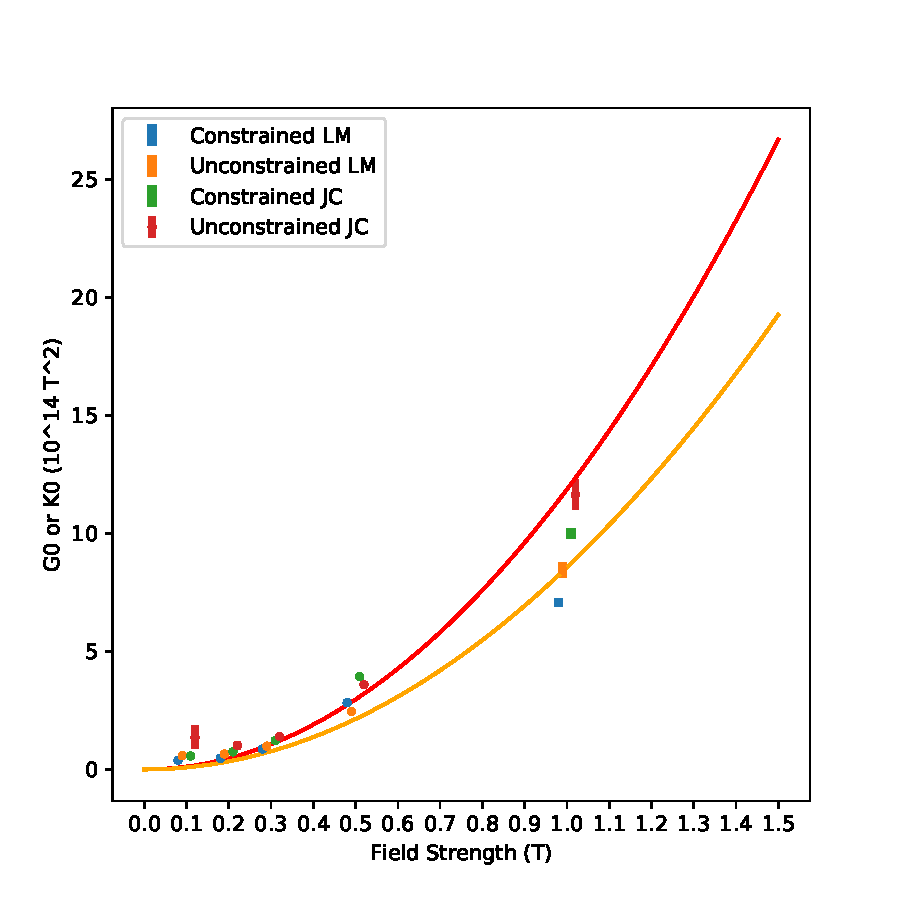
\includegraphics[width=10cm]{figures/diffmodels/G0K0field.pdf}
\caption[Field dependence of $G_0$ and $K_0$]{Field dependence of $G_0$ and $K_0$. Note points are moved on x-axis to better differentiate the series}
\label{fig:dm-KGfield}
\end{figure}

\begin{figure}[h!t]
  \makebox[\textwidth][c]{

  \begin{subfigure}[t]{0.6\textwidth}
  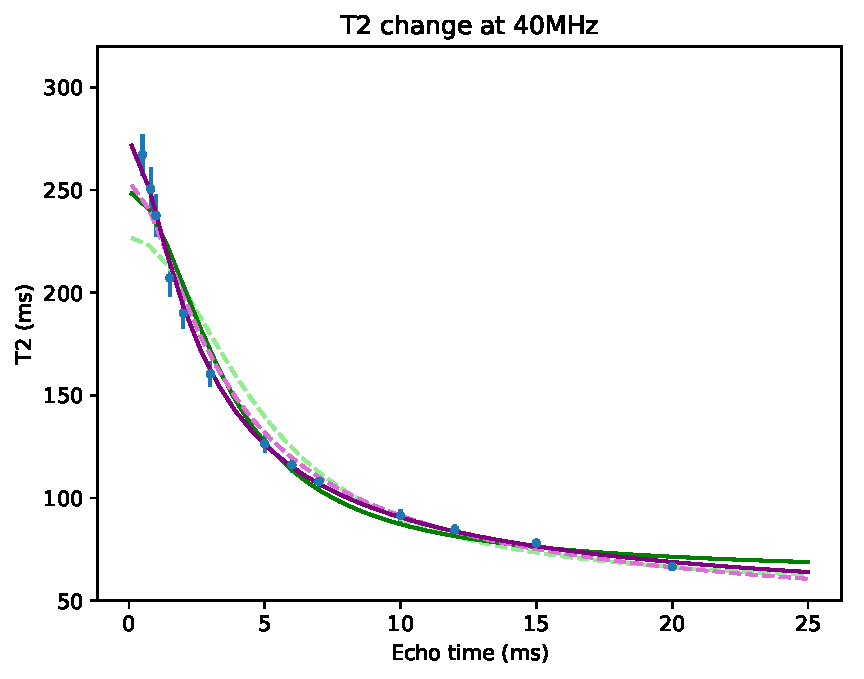
\includegraphics[width=\textwidth]{figures/diffmodels/40MHzT2.pdf}
  \caption{40 MHz: \SOtwo 2\%, Hct 0.35, v=1.0 cm/s}
  \label{fig:dm-fitResults40}
  \end{subfigure}
  \begin{subfigure}[t]{0.6\textwidth}
  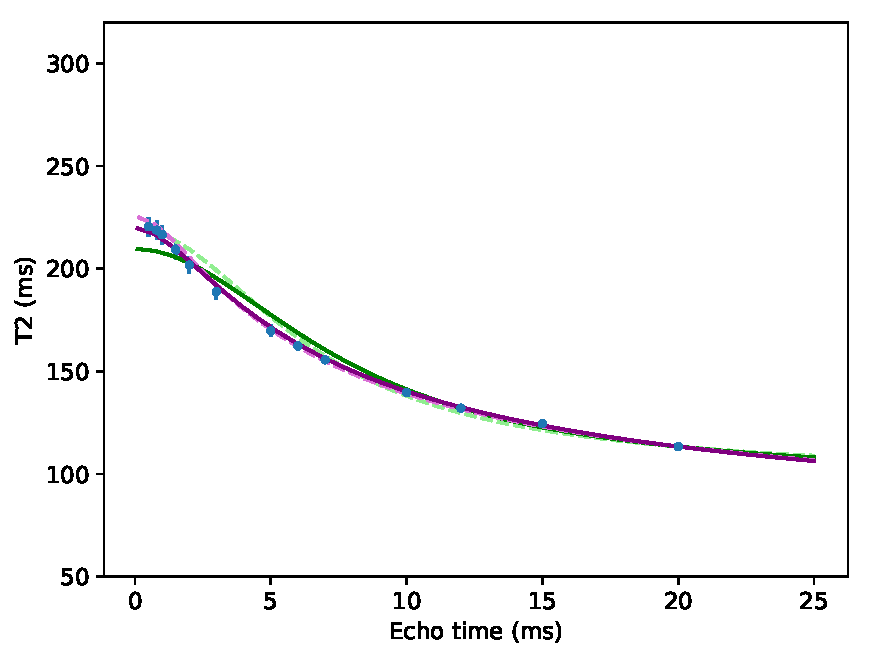
\includegraphics[width=\textwidth]{figures/diffmodels/20MHzT2.pdf}
  \caption{20 MHz: (\SOtwo 1\%, Hct 0.35, v=1.9 cm/s}
  \label{fig:dm-fitResults20}
  \end{subfigure}
  \hfill
  }

  \makebox[\textwidth][c]{
  \begin{subfigure}[t]{0.6\textwidth}
  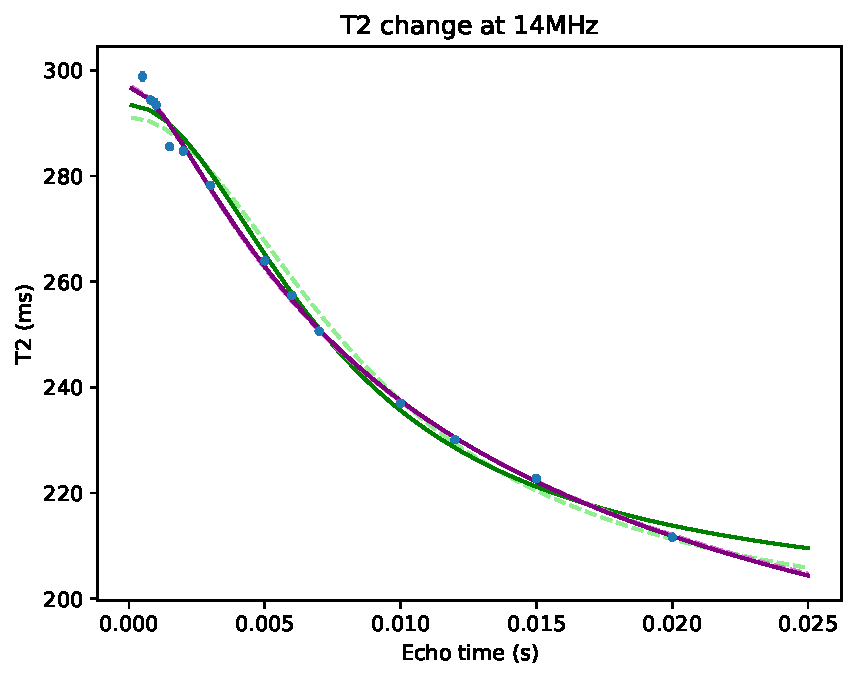
\includegraphics[width=\textwidth]{figures/diffmodels/14MHzT2.pdf}
  \caption{14 MHz: \SOtwo 5\%, Hct TODO iStat, v=1.1 cm/s}
  \label{fig:dm-fitResults14}
  \end{subfigure}
  \begin{subfigure}[t]{0.6\textwidth}
  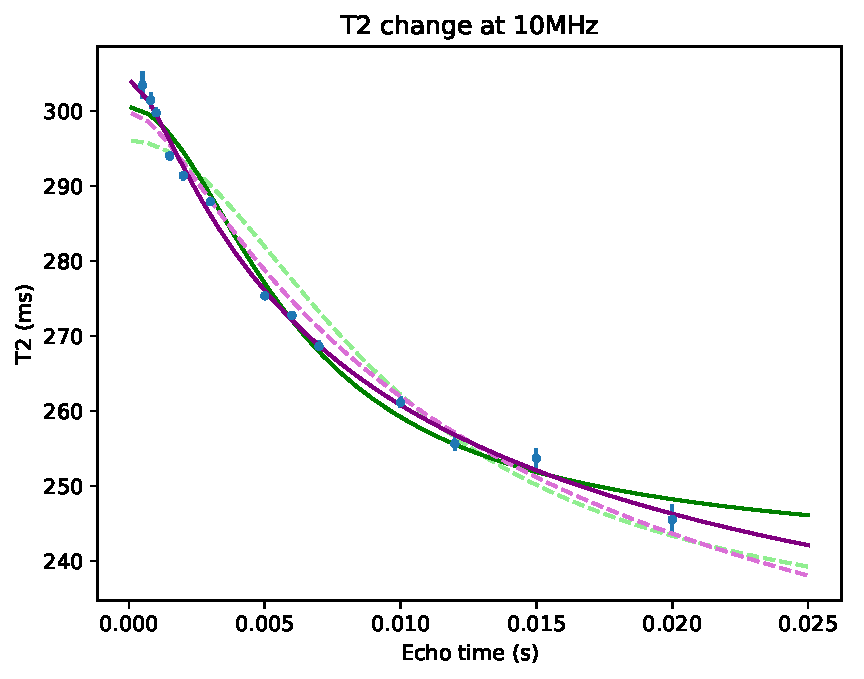
\includegraphics[width=\textwidth]{figures/diffmodels/10MHzT2.pdf}
  \caption{10 MHz: \SOtwo 2\%, Hct TODO iStat, v=1.6 cm/s}
  \label{fig:dm-fitResults10}
  \end{subfigure}
  \hfill
  }

  \makebox[\textwidth][c]{
  \begin{subfigure}[t]{0.6\textwidth}
  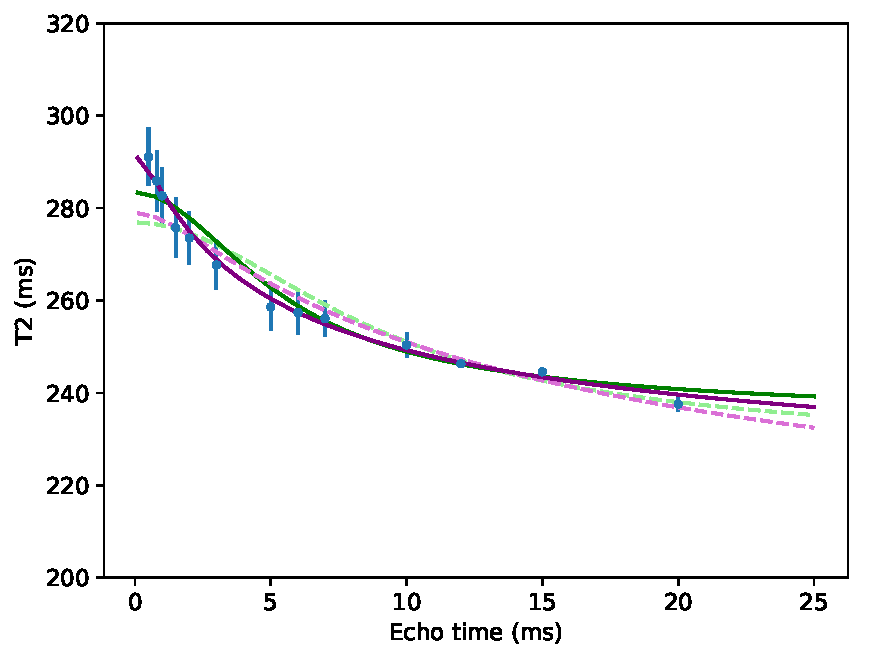
\includegraphics[width=\textwidth]{figures/diffmodels/5MHzT2.pdf}
  \caption{5 MHz: \SOtwo 7\%, Hct TODO iStat, v=2.5 cm/s}
  \label{fig:dm-fitResults5}
  \end{subfigure}
  \hspace{0.6\textwidth}
  }

  \caption[Luz-Meiboom and diffusion model fits at different fields]{Effect of changing echo time on \Ttwo at different fields, error bars show standard error (n=2). Best fit from Luz-Meiboom (Green) and diffusion model (Purple) are also shown. Dashed lines show constrained fits, while solid lines are unconstrained.}
  \label{fig:dm-fitResults}
\end{figure}

\section{Discussion}
These results show that the diffusion model of Jensen and Chandra tends to agree better with the measured data, even at low fields.
This is shown by the decreased SSR - the unconstrained JC fits provides much lower residuals than all other methods.
However, the curves / predictions of the LM model tend to be within 10 ms of the experimental data, which means that both models are probably fine TODO: more scientific??.
This is the same conclusion reached by Stefanovic and Pike and Chen and Pike, who found that the Luz-Meiboom exchange model provides acceptable accuracy at 1.5 T and at 3T respectively.

Additionally, with the exception of the 20 MHz results (where experiments were run after the 40 MHz run), the unconstrained fits produce concordant results of $\tau_{ex} = 2.17 \pm 0.06$ and $r_c = 3.58 \pm 0.08 um$ (weighted mean across field strengths).
This value for rc is within the range of red blood cell size, although it is smaller than the value found by Stefanovic (4.3 um)\cite{StefanovicHumanwholebloodrelaxometry2004}, and larger than the value found by Chen (2.7 um)\cite{ChenHumanwholeblood2009}.

This value for the exchange time is also within the range of results in the literature, although they do not correspond with the values measured at low field by Gomori\cite{GomoriNMRRelaxationTimes1987}.
This may be due to the long echo times they used, e.g. Gomori used two echo times of 32 and 64 ms at 0.94 T to get very short \Ttwo decays.
These long echo times were used because they were unable to get a good estimate of \Ttwo shortening at short echo times due to large uncertainties.
Looking at these long echo times may lead to greater sensitivity to exchange processes, and in particular, the 9.1 ms exchange time found by Gomori aligns well with literature values from permeability studies of the red blood cell membrane, which found values on the order of 10 ms.

Changes in the value of rc when moving from 40 MHz to 20 MHz are interesting, as it is known to be the same sample of blood.
This could reflect changes in the state of the blood, due to being cycled through the flow circuit for 4 hours previously. TODO check how long??
More precisely, the fitted parameter in \autoref{eq:JC} is actually $\frac{r_c^2}{2D}$, and it is possible that an increase in the fitted rc could also be due to a decrease in D, the diffusion coefficient.
It would be interesting to see if this effect occurs when there is no change in the magnetic field.

The \Kzero and \Gzero terms tend to follow a quadratic curve, which agrees with the predictions of theory \cite[Eq. 52-54]{JensenNMRrelaxationtissues2000}.
When extrapolating this to 1.5 T predicts a value of $G_0 = 26.7 \times 10^{-14}  T^2$.
This is about half of what is predicted using the results of Stefanovic, which (although based on studying changes in \SOtwo) can be used to find $G_0 = (45\pm0.51) \times 10^{-14} (sO_2)^2 = 40.6 \times 10^{-14}  T^2$ when using sO2=0.03, the average value from our experiments.
While the difference is significant, it is important to note that the variation between the oxygenations and haematocrit used at the different field strengths was not taken into account when fitting the data to find \Gzero, and multiple researchers \cite{StefanovicHumanwholebloodrelaxometry2004,ChenHumanwholeblood2009,GardenerDependencebloodR22010} have found that these parameters are correlated.

One possible weakness to these results is the effect of flow on the \Ttwo measurements.
It was shown in previous chapters that low amounts of flow through the circuit can cause decreases in the measured \Ttwo, without causing significant changes to the monoexponential decay in the CPMG experiment.
However, it is unclear whether the increasing echo time causes an increase in the strength of this effect, and whether it affects longer \Ttwo decays differently to shorter decays.
In these variable echo time experiments, this would be expected to cause underestimation \Ttwo values at longer echo times, which would lead to an overestimation in the magnitude of the \Ttwo shortening effect.
While the models still provide good agreement with the data points, it is unclear how the blood velocity affects the accuracy of the fitting parameters, as flow rate varied from 1 -- 2 cm/s between experiments.
Additionally, the flow rate has been assumed to be constant over the 5 minute course of the experiment.
This is relatively short compared to the longer term trends which were seen in the continuous flow experiments, so this should not have a significant effect.

As both models have acceptable predictions for the shape of the echo time curve, these results can not add more evidence of the actual physical mechanism of the \Ttwo shortening effect.
To be able to determine this, other experimental NMR techniques would need to be used such as chemical shift exchange sensitive methods (TODO what did Petrik actually call this?) that could detect this process directly.
Matwiyoff \cite{Matwiyofflineshapeswater1990} proposed that as the field decreased below 1.5 T, the exchange time would increase as the mechanism moved from mainly diffusion to mainly exchange.
This is the opposite to the trend observed here, where there a slight decreasing or constant trend in the exchange time, as field strength decreases.

Because of the variations between the measurements at different fields, with different samples of blood at each field, different amounts of time in the flow circuit, and variations in factors such as flow rate and oxygen saturation, it is difficult to make strong conclusions about the parameters underlying the models.
More data, with different samples of blood and better control of these experimental factors would need to be collected.
However, it is clear that both of the models are able to produce adequate agreement with experimental results.
